\documentclass[a4paper]{scrartcl}
\usepackage[cm]{fullpage}
\usepackage{amsmath, amssymb, esint}
\usepackage{siunitx}
\usepackage{braket}
\usepackage{isotope}
\usepackage{upgreek}
\usepackage[backend = biber, style = numeric-comp]{biblatex}

\usepackage{sectsty}
\sectionfont{\large\selectfont}
\subsectionfont{\normalsize\selectfont}

\usepackage{tikz, pgfplots}
\pgfplotsset{compat = 1.12}

\begin{filecontents}{\jobname.bib}
@online{NIST,
    title = {Nuclear Spins and Moments},
    date = {1976},
    url = {https://srd.nist.gov/JPCRD/jpcrd85.pdf}
}
\end{filecontents}
\addbibresource{\jobname.bib}

\begin{document}

\title{PHYS3111: Nuclear Magnetic Resonance Prework}
\author{ \\ \\}
\date{2017-05-01}
\maketitle

\section{Theoretical Questions}
It should be noted that all \(\omega\)s and \(\Omega\)s here have a hidden factor of \(\frac{1}{\hbar}\) that have been left out for clarity.

\subsection{Solve the matrix-eigenvalue equation \(\hat{s}_z \psi = s_z \psi\)}
Plugging the matrix \(\hat{s}_z = \frac{1}{2} \begin{pmatrix}1 & 0 \\ 0 & -1\end{pmatrix}\) into a CAS to solve for its eigensystem simply produces \(s_z = \frac{1}{2}\) when \(\psi = \begin{pmatrix}1 \\ 0\end{pmatrix} = \ket{\uparrow}\), and \(s_z = -\frac{1}{2}\) when \(\psi = \begin{pmatrix}0 \\ 1\end{pmatrix} = \ket{\downarrow}\)

\subsection{Solve the Schrodinger equation \(\hat{H} \psi = E \psi\) to find the eigenstates and energy levels of the Hamiltonian matrix \(\hat{H} = -\boldsymbol{\upmu} \cdot \mathbf{B} = -g \mu B_0 \hat{s}_z\)}
This is identical to the above question, but we simply have a extra factor of \(-g \mu B_0\). This simply results in energies of:
\begin{align*}
    E_{\ket{\uparrow}} &= -\frac{g \mu B_0}{2} \\
    E_{\ket{\downarrow}} &= \frac{g \mu B_0}{2}
\end{align*}

\subsection{Construct the Hamiltonian matrix where the magnetic field is now \(\mathbf{B} = B_{rf} \cos \omega t \:\hat{\mathbf{x}} - B_{rf} \sin \omega t \:\hat{\mathbf{y}} + B_0 \:\hat{\mathbf{z}}\)}
\begin{align*}
    \hat{H} &= -\boldsymbol{\upmu} \cdot \mathbf{B} \\
    &= -g \mu \hat{\mathbf{s}} \cdot \mathbf{B} \\
    &= -g \mu (B_{rf} \hat{s}_x \cos \omega t - B_{rf} \hat{s}_y \sin \omega t + B_0 \hat{s}_z) \\
    &= -\frac{g \mu}{2} \begin{pmatrix}
        B_0 & B_{rf} e^{i \omega t} \\
        B_{rf} e^{-i \omega t} & -B_0
    \end{pmatrix}
\end{align*}

\subsection{Show that if \(\Psi = a \:\hat{\mathbf{e}}_1 + b \:\hat{\mathbf{e}}_2\), \(\frac{\partial a}{\partial t} = \frac{i}{2} \left(\Omega b e^{i \omega t} + \omega_0 a\right)\) and \(\frac{\partial b}{\partial t} = \frac{i}{2} \left(\Omega a e^{-i \omega t} - \omega_0 b\right)\) satisfy the Schrodinger equation with the above Hamiltonian where \(\omega_0 = g \mu B_0\) and \(\Omega = g \mu B_{rf}\)}
With the above variables, our Hamiltonian now looks like:
\[\hat{H} = -\frac{1}{2} \begin{pmatrix}
    \omega_0 & \Omega e^{i \omega t} \\
    \Omega e^{-i \omega t} & -\omega_0
\end{pmatrix}\]
and its inverse is:
\[\hat{H}^{-1} = -\frac{2}{\Omega^2 + \omega_0^2} \begin{pmatrix}
    \omega_0 & \Omega e^{i \omega t} \\
    \Omega e^{-i \omega t} & -\omega_0
\end{pmatrix}\]

Let us first rearrange \(a\) and \(b\) such to eliminate the non-time derivatives of themselves from their expressions:
\begin{align*}
    a &= -\frac{2 i}{\Omega^2 + \omega_0^2} \left(\Omega e^{i \omega t} \frac{\partial b}{\partial t} + \omega_0 \frac{\partial a}{\partial t}\right) \\
    b &= -\frac{2 i}{\Omega^2 + \omega_0^2} \left(\Omega e^{-i \omega t} \frac{\partial a}{\partial t} - \omega_0 \frac{\partial b}{\partial t}\right) \\
    \therefore \Psi &= -\frac{2 i}{\Omega^2 + \omega_0^2} \begin{pmatrix}
        \Omega e^{i \omega t} \frac{\partial b}{\partial t} + \omega_0 \frac{\partial a}{\partial t} \\
        \Omega e^{-i \omega t} \frac{\partial a}{\partial t} - \omega_0 \frac{\partial b}{\partial t}
    \end{pmatrix} \\
    &= -\frac{2 i}{\Omega^2 + \omega_0^2} \begin{pmatrix}
        \omega_0 & \Omega e^{i \omega t} \\
        \Omega e^{-i \omega t} & -\omega_0
    \end{pmatrix} \begin{pmatrix}
        \frac{\partial a}{\partial t} \\
        \frac{\partial b}{\partial t}
    \end{pmatrix} \\
    &= i \hat{H}^{-1} \frac{\partial \Psi}{\partial t}
\end{align*}

Applying our Hamiltonian to this wavefunction:
\begin{align*}
    \hat{H} \Psi &= i \hat{H} \hat{H}^{-1} \frac{\partial \Psi}{\partial t} \\
    &= i \frac{\partial \Psi}{\partial t}
\end{align*}
which is our original Schrodinger equation. Since the substitutions did not lead to a contradiction, it must mean \(a\) and \(b\) satisfy the equation.

Solving this differential equation then gives us an explicit solution:
\begin{align*}
    a &= \left(a_0 \cos \frac{\omega' t}{2} + \frac{i}{\omega'} \left(b_0 \Omega + a_0 (\omega_0 - \omega)\right) \sin \frac{\omega' t}{2}\right) e^{\frac{i \omega t}{2}} \\
    b &= \left(b_0 \cos \frac{\omega' t}{2} + \frac{i}{\omega'} \left(a_0 \Omega - b_0 (\omega_0 - \omega)\right) \sin \frac{\omega' t}{2}\right) e^{\frac{-i \omega t}{2}} \\
    \omega' &= \sqrt{(\omega_0 - \omega)^2 + \Omega^2}
\end{align*}

\subsection{If the particle begins with spin up, find the probability of finding the particle in spin down as a function of time.}
Since our wavefunction is \(\Psi = a \ket{\uparrow} + b \ket{\downarrow}\), the probability of spin up and down are \(a^{\dag} a\) and \(b^{\dag} b\) respectively.

Since the particle begins with spin up, we have:
\begin{align*}
    a^{\dag} a \big|_{t = 0} &= 1 \\
    b^{\dag} b \big|_{t = 0} &= 0 \\
    \therefore a_0 = 1 \\
    b_0 = 0
\end{align*}

This results in a \(b\) and \(b^{\dag} b\) of:
\begin{align*}
    b &= \frac{i \Omega}{\omega'} e^{\frac{-i \omega t}{2}} \sin \frac{\omega' t}{2} \\
    b^{\dag} b &= \frac{\Omega^2}{\omega'^2} \sin^2 \frac{\omega' t}{2} \\
    &= \frac{\Omega^2}{(\omega_0 - \omega)^2 + \Omega^2} \sin^2 \frac{\omega' t}{2}
\end{align*}

\subsection{What parameter determines the width of the resonance?}
\begin{figure}
    \centering
    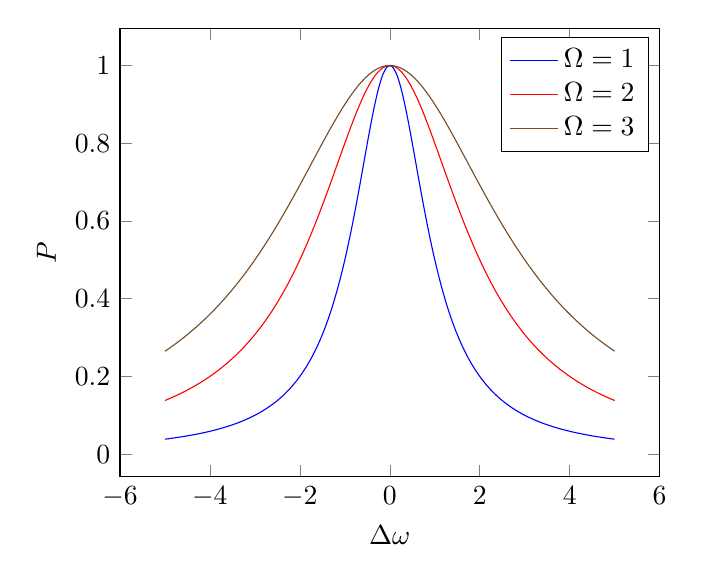
\begin{tikzpicture}
        \begin{axis}[
            xlabel = \(\Delta\omega\),
            ylabel = \(P\),
            samples = 100
        ]
            \addplot +[no marks, smooth, domain = -5:5] {1 / (x^2 + 1)};
            \addplot +[no marks, smooth, domain = -5:5] {4 / (x^2 + 4)};
            \addplot +[no marks, smooth, domain = -5:5] {9 / (x^2 + 9)};
            \legend{\(\Omega = 1\), \(\Omega = 2\), \(\Omega = 3\)}
        \end{axis}
    \end{tikzpicture}
    \caption{Resonance strength against \(\Delta\omega\)}
    \label{fig:resonance}
\end{figure}

From the previous question, we can see we have a probability of finding the particle spin down proportional to:
\[P = \frac{\Omega^2}{\Delta\omega^2 + \Omega^2}\]

This is plotted with various values of \(\Omega\) in Figure \ref{fig:resonance}. As can be seen, increasing \(\Omega \propto B_{rf}\) increases the width of the resonance.

\section{Experimental Questions}
\subsection{What are the proton and electron magnetic moments?}
CODATA 2014 gives the following values:
\begin{align*}
    \mu_p &= \SI{1.411e-26}{\joule\per\tesla} \\
    \mu_e &= \SI{-9.285e-24}{\joule\per\tesla}
\end{align*}

\subsection{Using these values, calculate the magnetic field \(B_0\) which would cause:}
\subsubsection{Protons to precess at \SI{14}{\mega\hertz}.}
\[B_0 = \frac{\omega_0}{\mu_p} = \frac{2 \pi \hbar f_0}{\mu_p} \approx \SI{657}{\milli\tesla}\]

\subsubsection{Electrons to precess at \SI{50}{\mega\hertz}.}
\[B_0 = \frac{2 \pi \hbar f_0}{\mu_e} \approx \SI{3.57}{\milli\tesla}\]

\subsection{Calculate the ratio of protons in the spin down state \(n_{\ket{\downarrow}}\) to the spin up state \(n_{\ket{\uparrow}}\) from the Boltzmann distribution with \(T = \SI{25}{\degreeCelsius}\) and \(B_0 = \SI{0.6}{\tesla}\).}
From question 1.2, we have an energy separation of \(\Delta E = g \mu B_0 = \mu_p B_0\).

From the Boltzmann distribution, we have:
\[\frac{n_{\ket{\downarrow}}}{n_{\ket{\uparrow}}} = e^{-\frac{\Delta E}{T k_B}} = e^{-\frac{\mu_p B_0}{T k_B}} \approx 0.999999\]

This means that under these conditions, the number of protons in the spin down state is only very slightly less than the ones in spin up.

\subsection{For a \isotope[19]{F} nucleus:}
\subsubsection{What is its magnetic moment?}
\[\mu_F = 2.6288 \mu_N = 2.6288 \frac{e \hbar}{2 m_p} \approx \SI{1.3278e-26}{\joule\per\tesla}\]\cite{NIST}

\subsubsection{Calculate the field strength in which it would precess at \SI{14}{\mega\hertz}.}
\[B_0 = \frac{2 \pi \hbar f_0}{\mu_F} \approx \SI{699}{\milli\tesla}\]

\subsubsection{Calculate its resonant frequency in the field found for protons earlier.}
\[f_0 = \frac{\mu_F B_0}{2 \pi \hbar} = \frac{\mu_F}{\mu_p} \SI{14}{\mega\hertz} \approx \SI{13.2}{\mega\hertz}\]

\printbibliography

\end{document}